\chapter{Analysis Steps}
\label{analysis}

The ultimate goal of this analysis consists of comparing 
ctapipe's geometric reconstruction method to the DISP-based approach,
that was implemented to improve results on low multiplicity events
and provide a base for monoscopic analyses.
This includes calculating the point source sensitivity curve
for each of the two analyses.
An exhaustive comparison would require to optimize all parameters,
that occur in the analysis steps from the low level monte carlo
data to the final sensitivity curve, independently for both approaches.
As this is not feasible, especially in the context of a master thesis, 
most analysis steps get performed in the same way, 
with parameters that showed good results in other analyses.

The multiple steps of the analysis will be explained in the following.
All parameters for the analysis aswell as the features used for the
different random forests can be found in appendix \ref{sec:app_params}.

\section{Simulated Data}
Monte carlo simulations are a crucial part to 
understand the behaviour of an experiment. 
Simulating the underlying physic and the response of the experiment
allows the testing of new algorithms aswell as improving the general understanding
of the physical processes at work. 
In this case, since CTA is not yet fully operational,
the analysis can not be based on real data at all.
Instead simulated data has to be used.

Monte carlo simulations for CTA are done using a combination of the
programs CORSIKA and sim\_telarray.
While CORSIKA handels the formation and propagation of air showers
in the atmosphere including the generated chernkov light,
the detector response is simulated using the software
sim\_telarray \cite{BERNLOHR2008149}.

The datasets are simulated and shared across the CTA collaboration.
The analysis in this thesis is based on the southern array simulations
from the PROD3 simulations \cite{ACHARYYA201935}. 
This production was done in order to define the final array layouts. 
For this reason the datasets include more telescopes, 
than the array will eventually have, in order to compare
different layouts and telescope positions.
For the analysis, the telescopes are chosen in a way, that
the resulting array resembles the final southern array (See section \ref{sec:cta}).

The data contains everything the telescopes would measure at a low level 
starting from uncalibrated waveforms in each pixel
plus additional MC information, that will not be present at real experiments.
This includes the simulated particle direction, energy and type.
This ground-truth allows to quantify the effectiveness of the 
algorithms by comparing the predictions with the true values.

Because not all the necessary information to reconstruct a recorded event 
changes with each shower and telescope, the data follows a certain hierarchie.
Some information is the same for a number of events, in the case of
a monte carlo simulation this includes the simulated particle spectrum
of the run amongst others.
Some information can not be considered to be the same for all events,
including the particles energy, type and direction. This holds for both
the true values and reconstructed features.
At last certain information about a single event is different between
the telescopes such as the recorded images.


% To adress a specific recorded event, the event information will be split into
% three layers, that get be saved as separate dataframes, denoted with the keys:
% \begin{enumerate}
%     \item{$runs$: This contains non-event-specific information about the monte carlo run, e.g.
%     spectral\_index, particle injection height, ...}
%     \item{$array\_events$: Any shower that triggered the array at some point 
%     is considered to be an array event.
%     Array-level features consist of array-wide shared event information 
%     (e.g. number of triggered telescopes, average intensity),
%     reconstructed high-level features of the primary particle (e.g. energy, source position) and the 
%     event specific monte carlo information to compare the reconstructed values against.}
%     \item{$telescope\_events$: This includes how a specific telescope has seen the shower and
%     contains information about the telescope itself (e.g. focal length). Telescope-level features 
%     describe the camera image and contain reconstructed features that were retrieved based on 
%     the telescope's specific measurements.}
% \end{enumerate}

In the following a separation into array-events and telescope-events is
taken in order to adress different levels of data.
The number of triggered telescopes in an array-event
after all analysis steps and cuts 
will be referred to as the event multiplicity.
This can differ from the original trigger multiplicity, 
for example if a telescope recorded an image, but the
image is found to not be useful for the analysis.
The latter is not used
in the analysis.

Different simulations are used for the analysis:
Diffuse gamma and proton events are used for the training of the models,
whereas the sensitivity evaluation is performed on point-like gamma and diffuse proton events.
The event counts are listed in table \ref{tab:datasets}.

\begin{table}
    \caption{Event counts for the different datasets in use.}
    \begin{center}
        \begin{tabular}{ l r r}
            %\hline
            Dataset & Array events & Telescope events \\
            \hline
            Diffuse gamma training set & 8\num{51671} & \num{3589934} \\
            Diffuse proton training set & 8\num{1166967} & \num{5031924} \\
            Diffuse proton test set & 8\num{3490562} & \num{15074461} \\
            Pointlike gamma test set & 8\num{955317} & \num{4554313} \\
        \end{tabular}
    \end{center}
    \label{tab:datasets}
\end{table}
% \subsection{Air Shower Simulation with CORSIKA}
% CORSIKA \cite{heck1998corsika} is the standard software to simulate different types of
% air showers in the field of astroparticle physics.
% It allows to choose primary particles at will and
% propagate them through the atmosphere, generating secondary particles, until
% eventually the ground is reached.
% Simulation options include, amongst other:
% \begin{itemize}
%   \item Amount of data to simulate
%   \item Several random seeds
%   \item Primary particle type
%   \item Range and slope of the energy spectrum
%   \item Alt/az range
%   \item Models and parameters for the electromagnetic and hadronic interactions
%   \item Models and parameters for the cherenkov light generation
%   \item Atmospheric properties, such as the magnetic field
%   \item Position and size of the detector grid
% \end{itemize}

% \subsection{Detector Simulation with sim\_telarray}
% sim\_telarray is a software developed for the HEGRA IACT experiment,
% but has since been developed to support arbitrary experiment setups \cite{BERNLOHR2008149}.
% % It is able to simulate the full detector response and can be used to either
% % perform complete simulations or use short-cuts in order to
% % improve on the computational efficiency.

% The main steps of the anaysis concern the optical raytracing of the cherenkov photons
% and the simulation of the readout electronics and triggers.

% The resulting data is meant to resemble the telescope raw data as closely as possible,
% be it digitized pulse shapes or integrated signal sums.

\section{Preprocessing with ctapipe}
The main processing pipeline for low-level CTA data is going to be ctapipe,
an open-source project hosted on github \cite{karl_kosack_2019_3372211}.
It is currently in development and not all the planned 
features are yet available.
Besides handling CTA-data, ctapipe also includes code to work with
other telescope geometries such as MAGIC.

At the time of writing, the latest stable version is 0.7
\cite{karl_kosack_2019_3372211}.
Because of the timeline of this thesis, the analysis is based
on version 0.6.2post178 \footnote{https://github.com/cta-observatory/ctapipe/commit/63fe206b1d603b0fff61486b6d0c18f73ef4e321}. 
This was the head of the master branch at the time
of finalizing the results.


\subsection{Telescope Level}
After recording an event, the data gets analyzed on telescope level,
meaning for each triggered telescope certain steps are performed
independently.

The recorded waveforms do not enter the analysis directly. Instead
an integration is performed first in order to extract a 2-dimensional
image for the event.
For this step an integration window has to be defined first.
In the chosen implementation an average waveform over all
neighbouring pixels gets calculated for each pixel.
The peak index of this average waveform then defines the center of the integration window.
The window width is a constant for each camera type.
Two values are then obtained per waveform:
The charge as the summed values and the pulse time as the index at which half
of the total charge is measured.
Figure \ref{fig:shower_raw} illustrates these values as two separate images in
the focal plane of the LST camera.
One can visually see the shower in the upper right quadrant of the
image by the higher photon count and the correlated pulse times.

\begin{figure}
	\centering
	\captionsetup{width=0.9\linewidth}
	\begin{subfigure}{.45\textwidth}
  		\centering
  		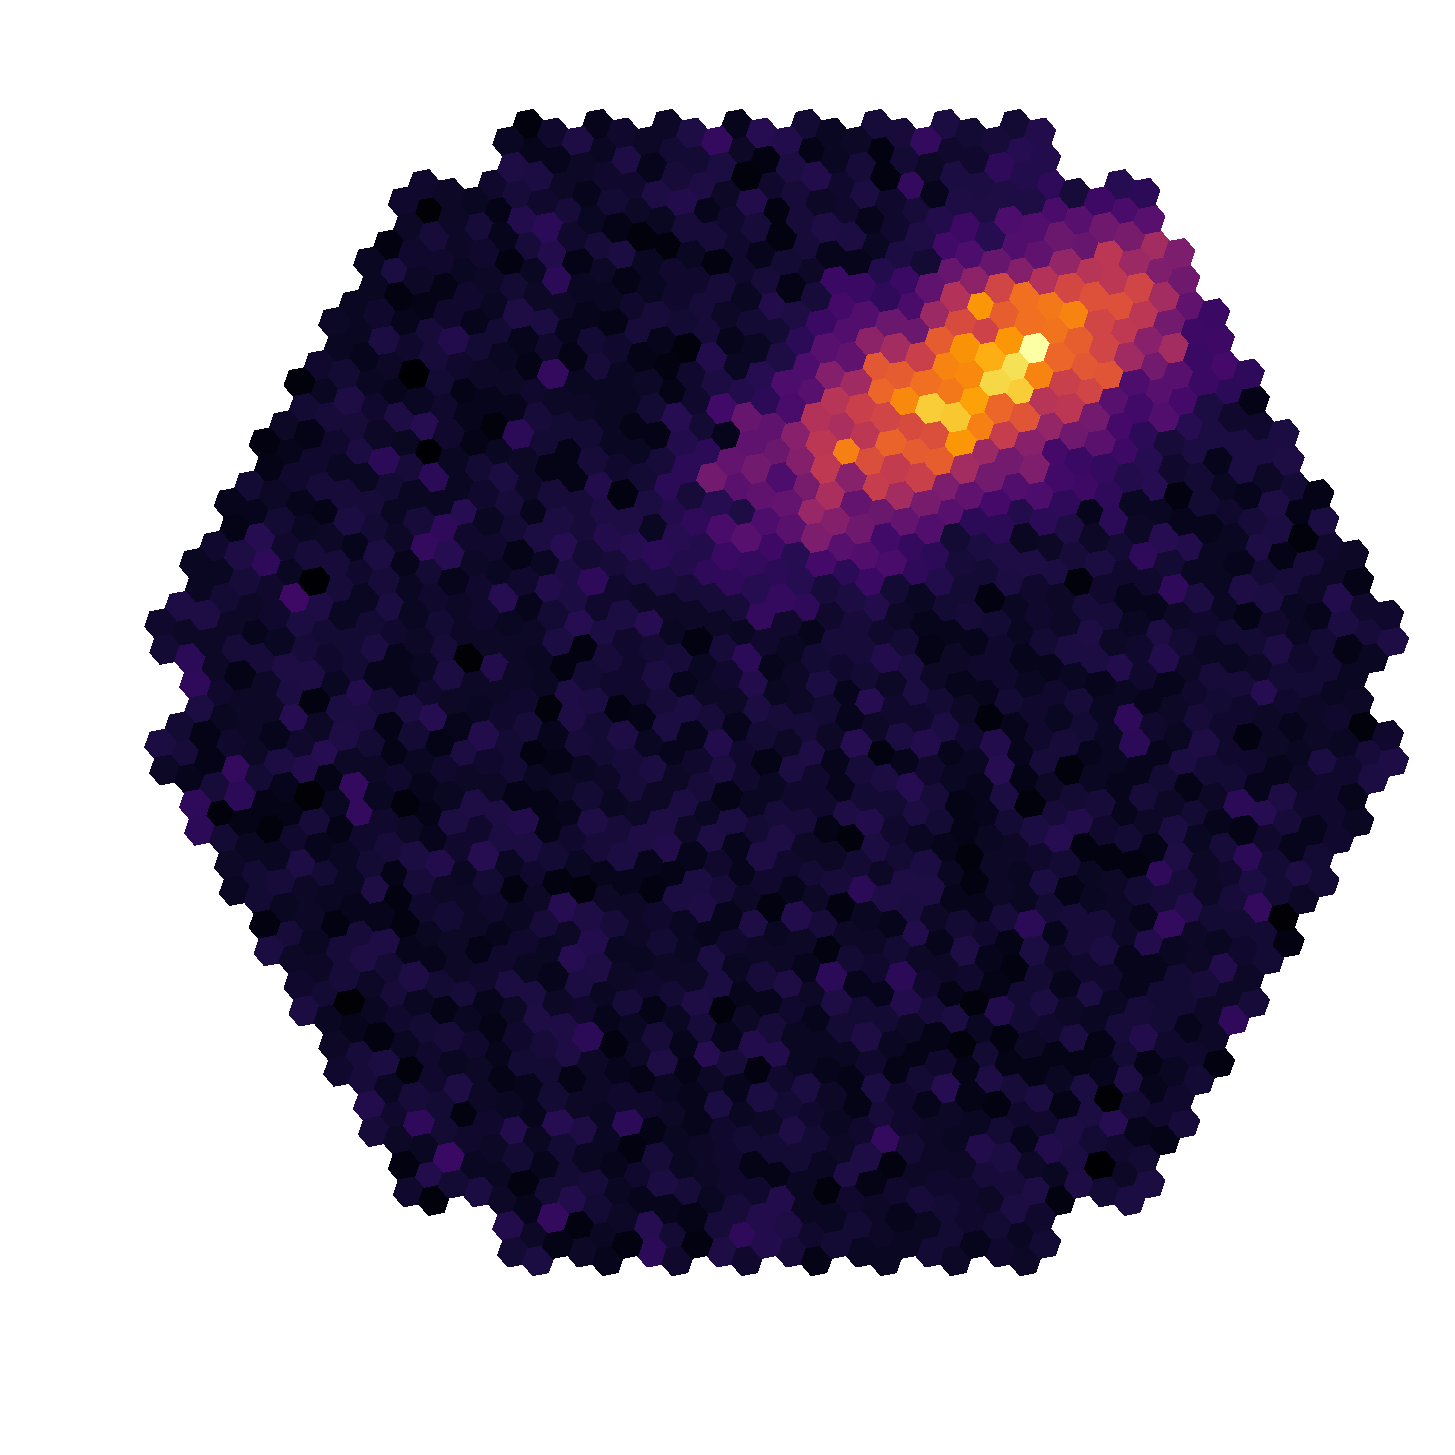
\includegraphics[width=\linewidth]{Plots/hillas_raw.pdf}
	\end{subfigure}%
	\begin{subfigure}{.45\textwidth}
 		\centering
		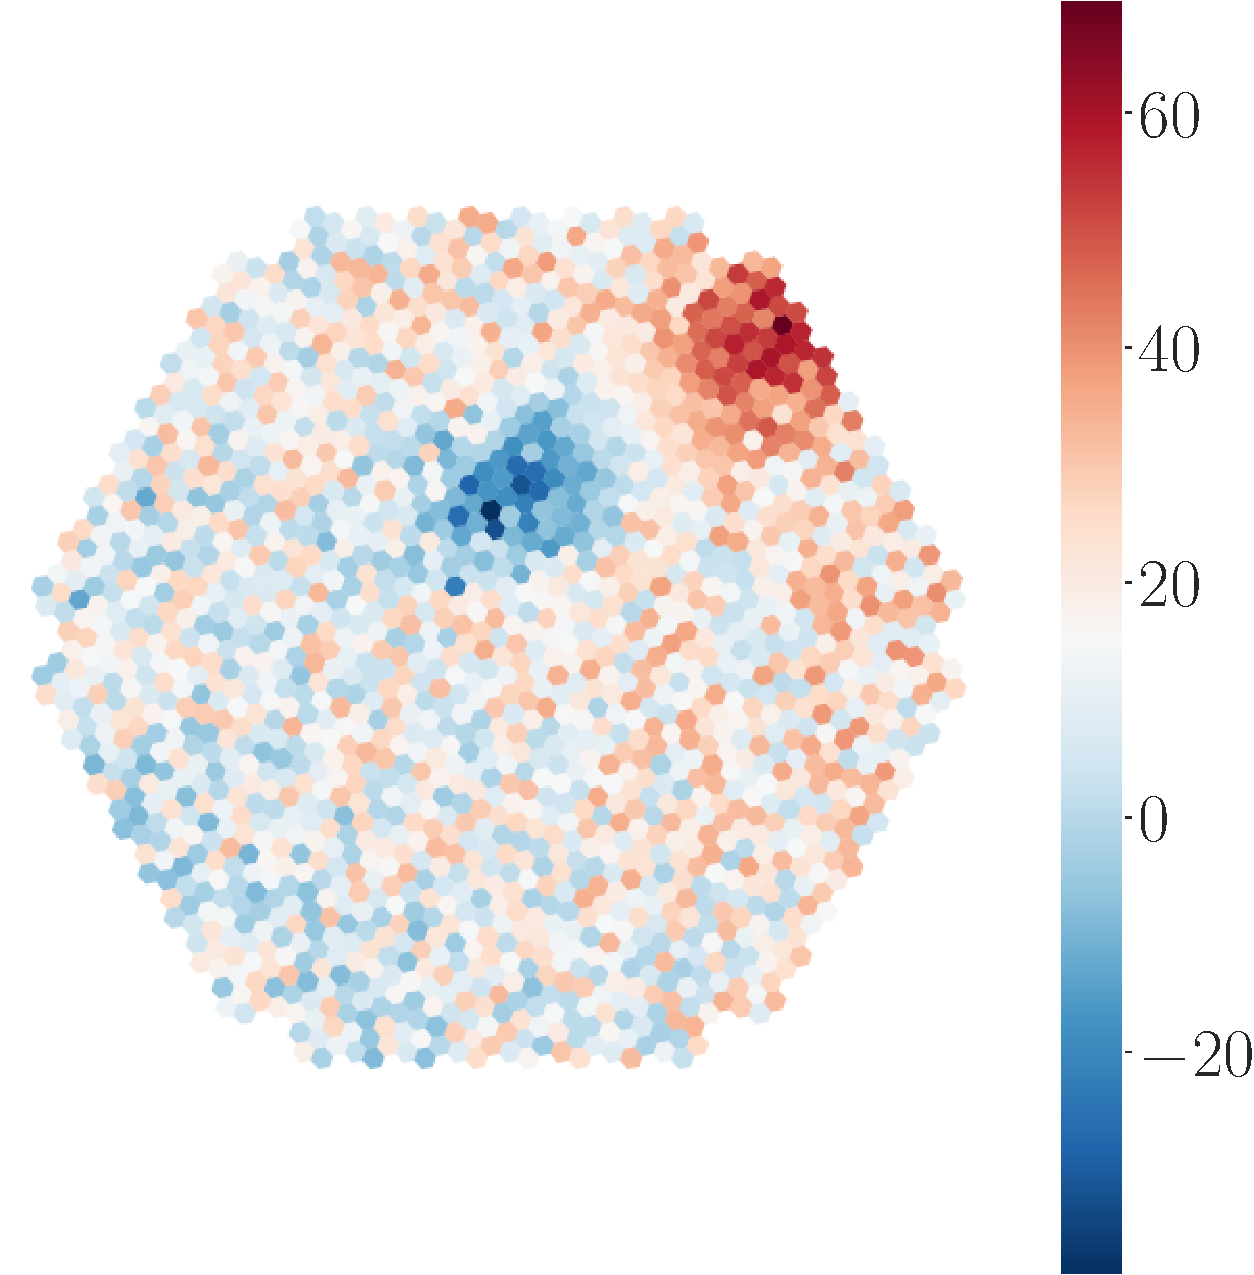
\includegraphics[width=\linewidth]{Plots/hillas_raw_time.pdf}
	\end{subfigure}
	\caption{
		Left: Extracted photon charge after waveform integration.
        The non-signal pixels contain a lot of noise. \\
		Right: Extracted pulse times after waveform integration.
        The shower pixels are highly correlated, whereas the background pulse times
        are uniformly distributed.}
	\label{fig:shower_raw}
\end{figure}


The resulting images then get cleaned to select the pixels,
that get used for further analysis.
The used algorithm works with two thresholds based on the 
pixel charge and one threshold defining the number of needed neighboring pixels.
In the first step, all pixels above the upper threshold with a set amount of neighbouring 
pixels above the neighbor threshold get selected.
In the second step, all pixels above the lower threshold with the same set amount of neighbouring pixels
above the upper threshold get added aswell.
Figure \ref{fig:shower_cleaning} illustrates the results on the sample shower shown before.
The parameters used for the cleaning are chosen relatively soft. This leads to
additional, smaller clusters in the image.
During the course of this thesis, I added an alternative algorithm, that is used by the FACT-collaboration 
and additionaly makes use of the pulse time information.
It works in a similar way, but with additional steps removing pixels, that arrived
at distant times, and multiple steps removing isolated pixels.
Because of the high effort needed to obtain optimal cleaning parameters,
no substantial performance gains could be found and the algorithm described above was 
used in order to make the results more comparable and avoid additional sources of errors.

\begin{figure}
	\centering
	\captionsetup{width=0.9\linewidth}
	\begin{subfigure}{.45\textwidth}
  		\centering
  		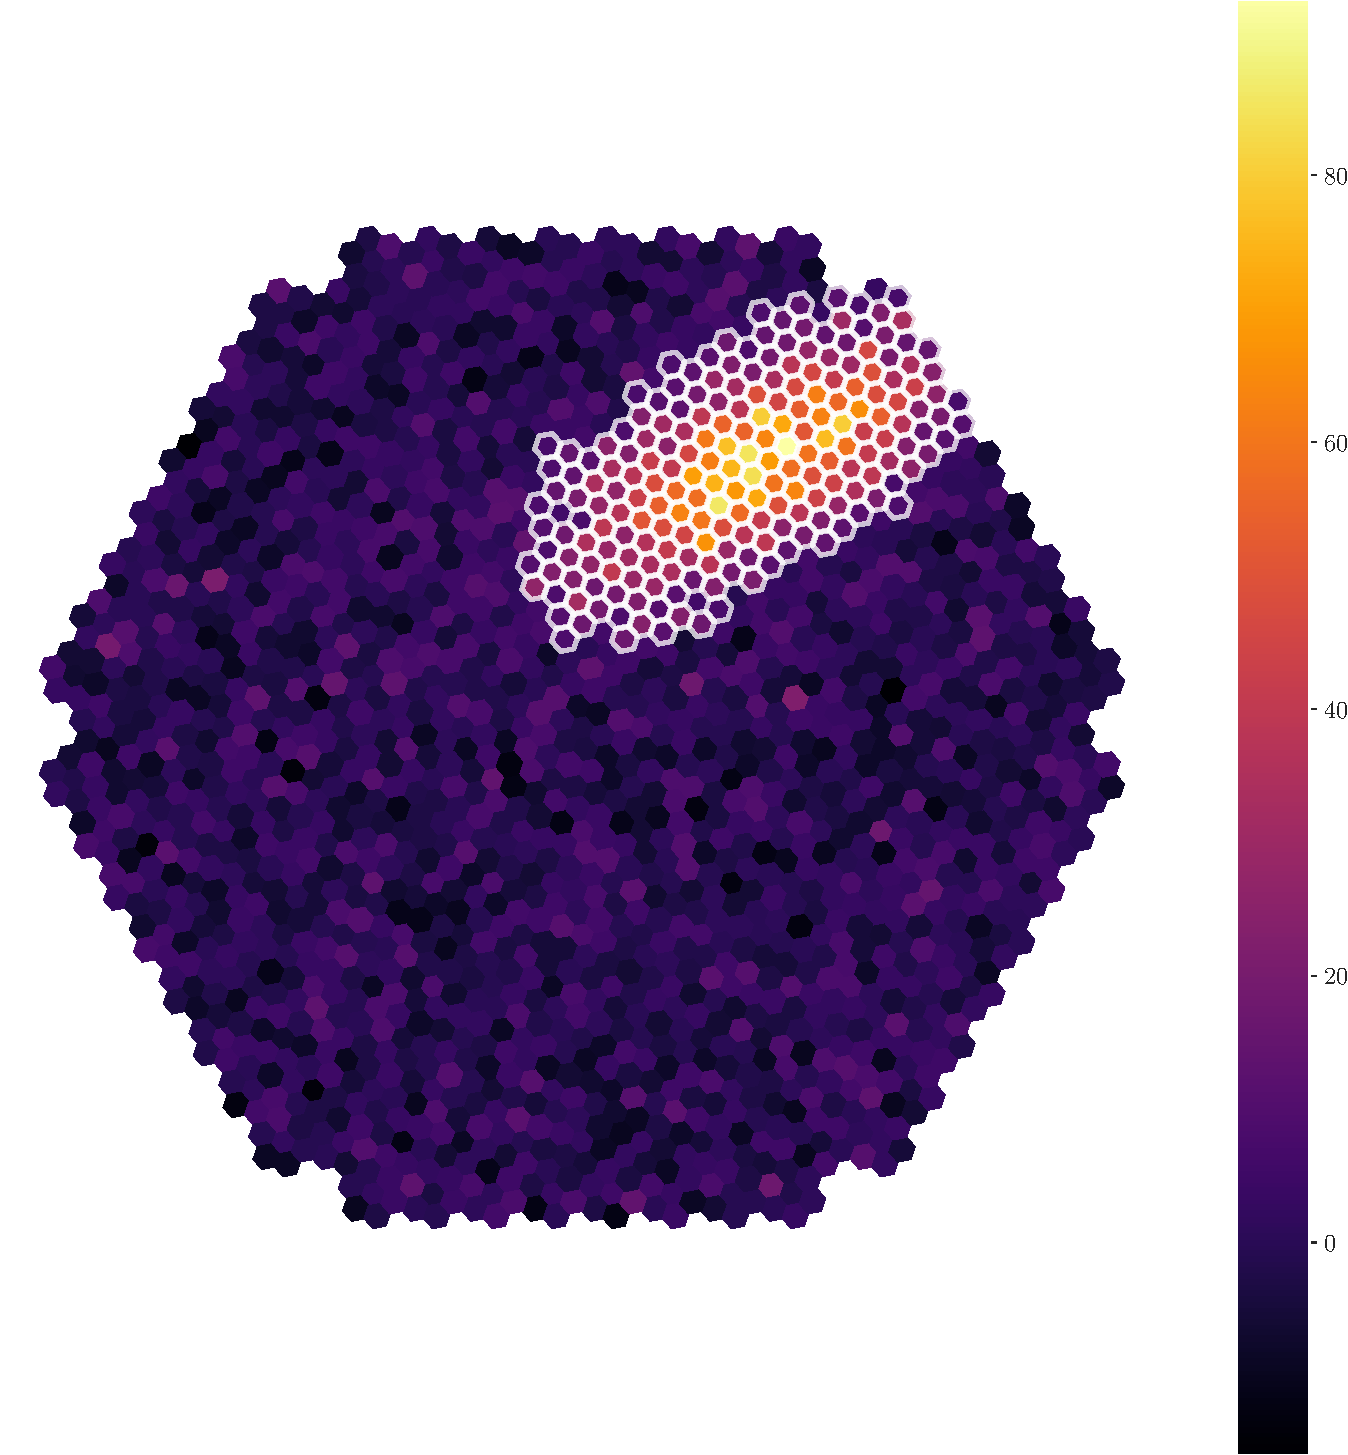
\includegraphics[width=\linewidth]{Plots/hillas_cleaned.pdf}
	\end{subfigure}%
	\begin{subfigure}{.45\textwidth}
 		\centering
		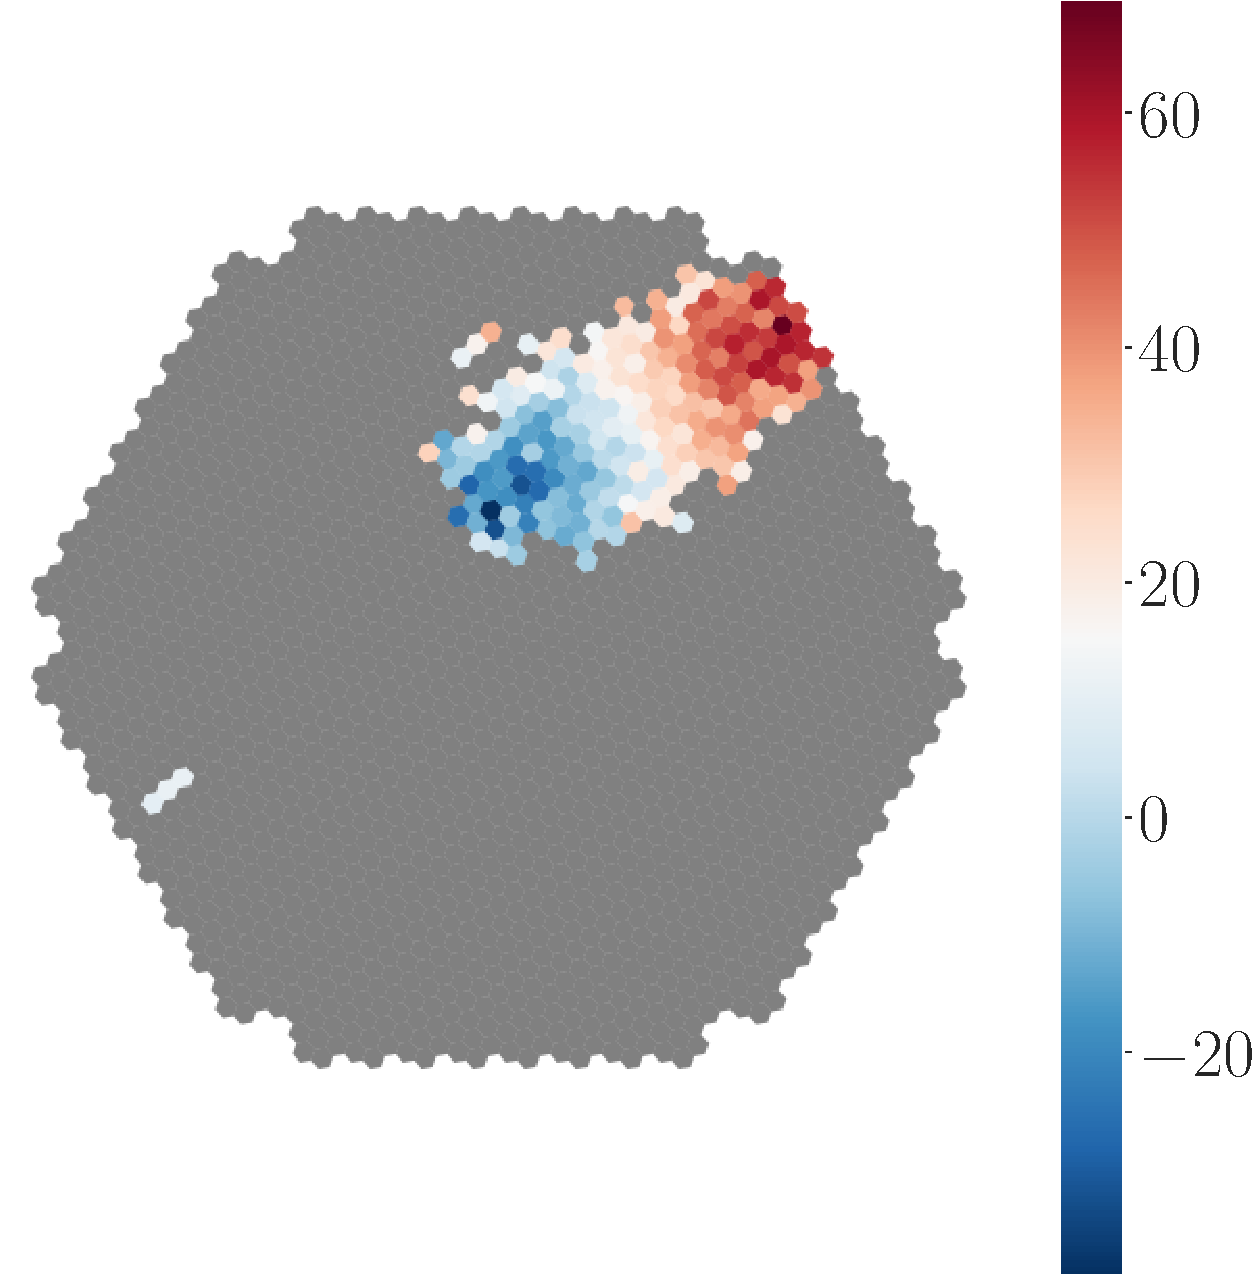
\includegraphics[width=\linewidth]{Plots/hillas_cleaned_time.pdf}
	\end{subfigure}
	\caption{
		Left: Shower image after applied cleaning. The cleaning is relatively soft,
        leaving two smaller pixel islands. Not seected pixels are marked in gray.\\ 
		Right: Pulse times after applied cleaning.}
	\label{fig:shower_cleaning}
\end{figure}

Several parameters can be calculated on the charge values, the most prominent ones are the 
hillas parameters, shown in figure \ref{fig:hillas_params}.
They are obtained via a principal component analysis (PCA) of the shower image
and are often times illustrated with an ellipse on top of the shower image.
The first (\enquote{main shower axis}) and second component are therefore
identified with the major and minor axis of an ellipse.

\begin{figure}
	\centering	
	\captionsetup{width=0.9\linewidth}
	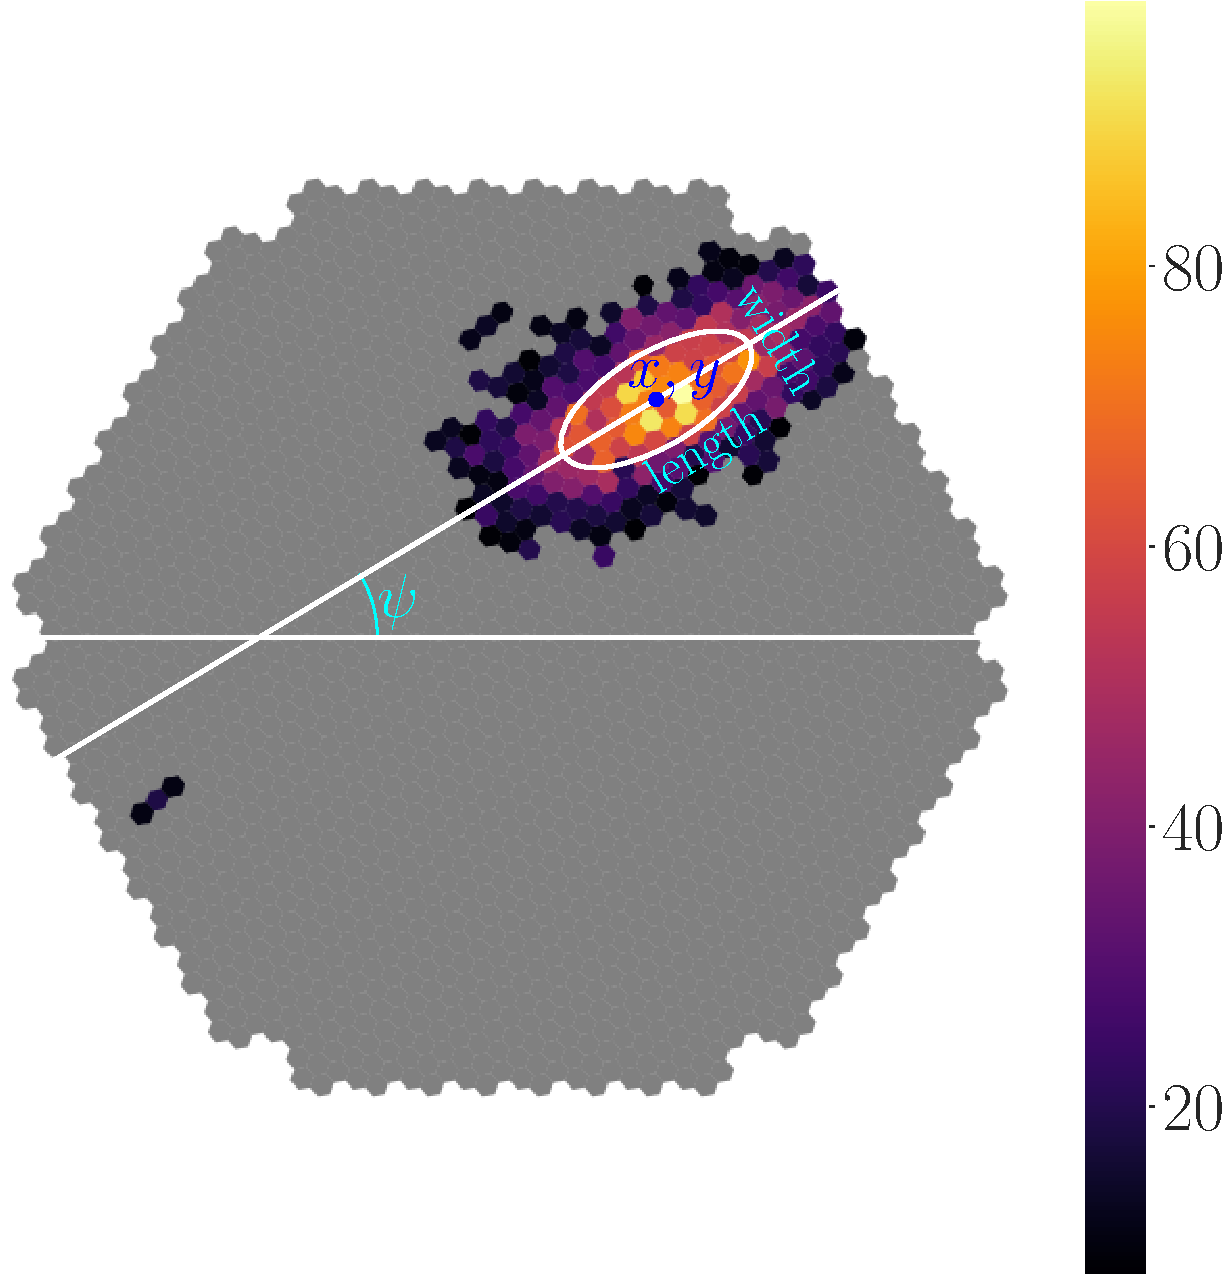
\includegraphics[width=.6\textwidth]{Plots/hillas_cleaned_params.pdf}
	\caption{The same cleaned shower-image as in figure \ref{fig:shower_cleaning}
	with the hillas-parameters calculated and marked in the camera frame.
	The parameters \texttt{Psi}, \texttt{x} and \texttt{y} describe the 
	orientation and position of the shower ellipse in the camera frame.
    The lengths of the PCA components are identified with the axes of
    an ellipse and named \texttt{length} and \texttt{width} for further
    reference.}
	\label{fig:hillas_params}
\end{figure}

Other parameters include variations of the leakage and concentration of the shower image.
Leakage describes how much of the signal is located in the outermost pixels of the camera
and thus gives a measure of how much light might have missed the camera.
Concentration describes how much of the measured charge is concentrated in a set of selected pixels.

In addition, I implemented an algorithm, that counts the separated clusters in the image,
the sum of which is referred to as number of islands. Depending on the applied 
cleaning, this can help separating gamma and hadron showers.

A class of parameters, that is evaluated on the pulse times, are the timing
parameters. These describe the temporal evolution of the image by fitting
a linear function on the pulse times. The parameters of the fit and the deviation
between observed and estimated pulse times are saved as the timing parameters.
Signal pixels should be highly correlated, whereas background noise 
is assumed to arrive at random times.

In total, the following parameters are calculated for each telescope event:

\textbf{Hillas Parameters:}

\begin{itemize}
    \item{\texttt{x, y}: Position of the center of gravity in cartesian coordinates.}
    \item{\texttt{Phi, r}: Position of the center of gravity in polar coordinates.}
    \item{\texttt{Psi}: Orientation of the main shower axis.}
    \item{\texttt{length, width}: Eigenvalues of the PCA.}
    \item{\texttt{intensity}: Summed charge in the image.}
    \item{\texttt{skewness, kurtosis}: Third order moments of the charge distribution along the main shower axis.}
\end{itemize}

\textbf{Leakage:}

\begin{itemize}
    \item{\texttt{leakage\_1\_intensity}: Percentage of photo-electrons in the outer most ring of pixels with respect to the photo-electrons in the whole image}
    \item{\texttt{leakage\_1\_pixel}: Percentage of pixels in the outer most ring of pixels with respect to the pixels in the whole image}
    \item{\texttt{leakage\_2\_intensity}: Percentage of photo-electrons in the two outer most rings of pixels with respect to the photo-electrons in the whole image}
    \item{\texttt{leakage\_2\_pixel}: Percentage of pixels in the two outer most rings of pixels with respect to the pixels in the whole image}
\end{itemize}

\textbf{Concentration:}

\begin{itemize}
    \item{\texttt{concentration\_cog}: Percentage of photo-electrons in the three pixels closest to the cog with respect to the photo-electrons in the whole image}
    \item{\texttt{concentration\_core}: Percentage of photo-electrons inside the hillas ellipse with respect to the photo-electrons in the whole image}
    \item{\texttt{concentration\_pixel}: Percentage of photo-electrons in the brightest pixel with respect to the photo-electrons in the whole image}
\end{itemize}

\textbf{Timing Information:}

\begin{itemize}
    \item{\texttt{slope, slope\_err}: Slope and corresponding uncertainty of a linear regression to the pixel-wise pulse times along the main shower axis.}
    \item{\texttt{intercept, intercep\_err}: Intercept and corresponding uncertainty of a linear regression to the pixel-wise pulse times along the main shower axis.}
    \item{\texttt{deviation}: Root-mean-square deviation between the individual pulse times and the predicted pulse times
        retrieved via the linear regression.}
\end{itemize}

\textbf{Other:}

\begin{itemize}
    \item{\texttt{num\_islands}: Number of individual clusters in the cleaned image.}
    \item{\texttt{num\_pixel\_in\_shower}: Number of pixels that survived the cleaning.}
\end{itemize}


\subsection{Array Level}
From the image descriptions high level features can be calculated,
that describe the primary particle.
Since CTA is going to be a stereoscopic experiment,
the information of multiple telescopes can be combined toweighted
reconstruct these properties.

At the time of the analysis, ctapipe is only able to give an estimation
of the shower impact, the primary particle interaction height and
the shower origin.

An algorithm, that makes use of the stereoscopic array planned for CTA
works based on the hillas parametrisation of the images:
For each triggered telescope, a 2D-plane is drawn into the spatial 3D-space
based on the main shower 
axis and the telescope orientation. These planes intersect and 
the weighted average of all intersections yields the 
orientation of the observed shower.
Weights are calculated as 
$$
\texttt{intensity} \cdot \texttt{length} / \texttt{width},
$$
putting more emphasis on bright images with high elongation.

Combining the main shower axes on the ground frame
and calculating the closest point to a common intersection
via the least squares method leads to 
an estimation of the impact point of the shower.
In addition the main interaction point can be caculated 
d by transforming the image cogs into the horizon frame and 
then the euclidian space.
This leads to lines between a telescopes position and the assumed
interaction point. The closest mutual point to all lines
then gets calculated with the least squares method again.

Inside of ctapipe, the HillasReconstructor combines the
above mentioned methods for the stereoscopic reconstruction of the
shower origin, interaction height and impact point.
For a general illustration see figure \ref{fig:hillas_reconstructor}.

% Since this method inherently requires a stereoscopic experiment
% and multiple triggered telescopes, it will not work for a single telescope.

\begin{figure}
	\centering
	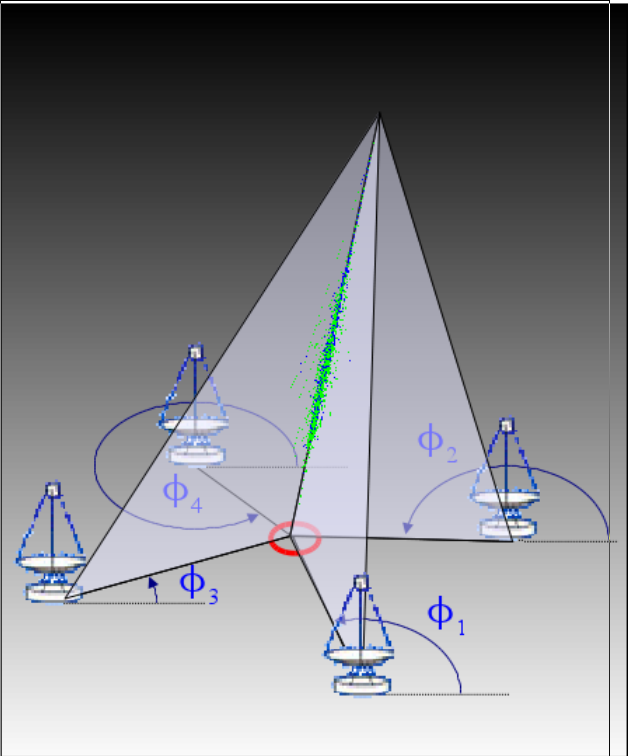
\includegraphics[width=0.6\textwidth]{images/hillas_reco.png}
	\caption{Illustration of a stereoscopic reconstruction of the shower impact.
    From each telescope a plane is drawn, the direct intersection 
    on the ground leads to the impact point (red circle).
    Not included is the reconstruction of the main interaction point
    and source position \cite{hillas_reco}.}
	\label{fig:hillas_reconstructor}
\end{figure}

This step leads to the following features on array level:
\begin{itemize}
    \item{\texttt{alt, az}: Reconstructed source position}
    \item{\texttt{core\_x, core\_y}: Reconstructed core position on the ground}
    \item{\texttt{average\_intensity}: Mean intensity over all triggered telescopes}
    \item{\texttt{h\_max}: Reconstructed main interaction height}
\end{itemize}
and the \texttt{distance\_to\_reconstructed\_core\_position}
on telescope level.

The error of the reconstructed shower origin $\Theta$ is defined
as the great circular distance between the reconstructed and true source position.
For the calculation, astropy and ctapipe use the Vincenty formula \cite{geodetic1975direct}.


\section{Event Reconstruction using Machine Learning}
With a lot of features calculated and high amounts of monte carlo
data available, (supervised) machine learning algorithms can perform
very well in these kind of analyses.
This analysis makes use of random forests for 
the background separation, energy estimation and an alternative reconstruction 
of the shower origin.

In the task of supervised machine learning, a model is trained on a
dataset with full information available.
Training in this context means to optimize the parameters of a 
model to minimize the error of the prediction on the training data.
The trained model can then later be used to estimate features on a dataset, which
lacks the needed information.

We define a dataset as having a number of samples with a fixed number of
features each. In the following we split
the features of our dataset into a set of input variables $\mathbf{X}$ and
a set of output variables $\mathbf{y}$.
The naming convention for
these sets follows the one of scikit-learn
\cite{scikit-learn}, \cite{sklearn_api}.
Other terminologies for the two feature sets include
predictors or independent variables for the input, and
responses or dependent variables for the output.

Training and applying the models to the data is based on the use of
the aict-tools package \cite{aict-tools} which itself makes use of
scikit-learn for the implementation of the machine learning algorithms.
The aict-tools have originally been developed for the FACT-experiment
which is a single IACT. 
Model feature importance is calculated
based on the scikit-learn functionality, which
uses the mean decrease impurity.
For a more general discussion on feature importance estimations see \cite{hastie2017springer}.

\subsection{Classification}
In (supervised) classification, the task is to predict of which of some
predefined classes the given sample is a member. The possible solutions for $y$
are from a discrete set of values in
contrast to a regression problem with a continuous solution space.
A model that performs classification on data is referred to as a
classifier.

The simplest case of classification problems
is \textit{binary classification} \cite{sokolova2009systematic},
which is also what is needed for this analysis.
In this case only two distinct
classes exist.
% A common example for a classification problem is an Email spam filter,
% where mails get categorized in at least two categories based
% on their content and meta data \cite{DBLP:journals/corr/cs-CL-0006013}.

For binary classification, a set of measures
to define the quality of the prediction can be defined, starting with the confusion matrix
shown in table \ref{tab:confusion},
with $pos$ referring to the true label of the positive (i.e. signal)
and $neg$ referring to the label of the negative (i.e. background) class.

\begin{table}
    \caption{Definition of the confusion matrix for binary classification.
    The main diagonal includes the correct predictions, wrong predictions are on the off diagonal.}
    \begin{center}
        \begin{tabular}{ l| l l}
            %\hline
            {} & Predicted as $pos$ & Predicted as $neg$ \\
            \hline
            $pos$ & true positive ($tp$) & false negative ($fn$) \\
            %\hline
            $neg$ & false positive ($fp$) & true negative ($tn$) \\
            %\hline
        \end{tabular}
    \end{center}
    \label{tab:confusion}
\end{table}

An ideal classification would result in
\begin{equation*}
  fp = fn = 0.
\end{equation*}

As this can usually not be achieved, different measures
can be used to examine the classifiers performance
depending on the goal of the analysis.
Some of the more common ones are listed in table \ref{tab:class_metrics}.

\begin{table}
    \caption{Popular metrics for binary classification tasks.}
    \begin{center}
        %\caption{
         % Common metrics for classification tasks, taken from \cite{sokolova2009systematic}.}
        \begin{tabularx}{\textwidth}{l c X}
            %\hline
            Measure & Formula & Interpretation \\
            \hline
            Accuracy & $\frac{tp+tn}{tp+fn+fp+tn}$ & Class agreement on both labels \\
            Balanced Accuracy & $\frac{1}{2}(\frac{tp}{tp+fn}+\frac{tn}{fp+tn})$ & Improved accuracy for unbalanced class distributions \\
            Precision & $\frac{tp}{tp+fp}$ & Class agreement with the positive labels given by the classifier \\
            Recall/Sensitivity & $\frac{tp}{tp+fn}$ & Effectiveness of a classifier to identify positive labels \\
            F$_{\beta}$-score & $\frac{(\beta^2+1)tp}{(\beta^2+1)tp+\beta^2fn+fp}$ & Weighted harmonic mean between precision and recall with choosable weight $\beta$ \\
            Specificity & $\frac{tn}{fp+tn}$ & How effectively a classifier identifies negative labels \\
        \end{tabularx}
    \end{center}
    \label{tab:class_metrics}
\end{table}

A classifier can also be used to predict a class probability.
For the case of binary classification, this can be a number between 0 and 1,
with 0 being one class and 1 being the second.
The classifier threshold is then the value at which the separation into the two classes happens.
One can then calculate the Area Under the Receiver Operating Characteristic curve (AUC).
The ROC-curve is gained by plotting the true positive rate against the false positive rate while varying the classifier threshold.
The area under the (normalised) ROC-curve is thus a measure for whether the classifier will
rank a randomly chosen positive sample higher than a randomly chosen negative sample \cite{FAWCETT2006861}.


\subsection{Regression}
Regression is the task of predicting a continuous variable
from a set of input variables.
The simplest approach
to this problem is the ordinary linear least squares method,
which minimizes the Mean Squared Error (MSE).
Other metrics for regression tasks include the
Mean-Absolute-Error (MAE)
or the Coefficient of Determination ($R^2$), all of which are listed in table
\ref{tab:regr_metrics}.

% Given an unrestricted linear model
% \begin{align}
% 	y &= X\beta + e \\
% 	E(y) &= X\beta \\
% 	Cov(y) &= \sigma^2 I_n
% \end{align}
% with a measured vector $y$, the design matrix $X$,
% an unknown parameter vector $\beta$, a random error $e$
% and pairwise orthogonal features $y_i$,
% the least-squares solution is given by the solution of
% the minimizing problem in equation \ref{eq:min_least_squares}.

% \begin{equation}
% 	\min_{\beta\in\mathbb{R}^k} \lVert y - X\beta \rVert
% 	\label{eq:min_least_squares}
% \end{equation}

% If $(X^TX)^{-1}$ exists, the unique solution for the
% least square estimation of $\beta$ becomes:
% \begin{equation}
% 	\hat{\beta} = X^+ y,
% \end{equation}

% with the Moore-Penrose inverse $X^+ = (X^TX)^{-1}X^T$.
% The estimation of $y$ is then:
% \begin{equation}
%   \hat{y} = X\hat{\beta}.
% \end{equation}

% The metric, that is minimized by the least-squares solution
% is the Mean Squared Error (MSE).



\begin{table}
  \caption{Popular metrics for a regression problem with $n$ samples.}
  \begin{center}
    \begin{tabularx}{\textwidth}{l c X}
      Measure & Formula & Interpretation \\
      \hline
      Mean squared error & $\frac{1}{n}\sum_i^n |y_i-\hat{y_i}|$ & Prediction error disregarding the direction of over- and underprediction \\
      Mean absolute error & $\frac{1}{n}\sum_i^n (y_i-\hat{y_i})^2$ & For an unbiased predictor: Variance of the regressor. Heavily weights outliers. \\
      Coefficent of Determination & $1 - \frac{\sum_i^n (\bar{y_i}-\bar{y})^2}{\sum_i^n (y_i-\bar{y})^2}$ & Share of observed variance that is explained by the model.\\
    \end{tabularx}
  \end{center}
  \label{tab:regr_metrics}
\end{table}

Many metrics closely connected to these metrics exist, such as the root mean squared error (RMSE)
or the mean absolute percentage error (MAPE).

\subsection{Decision Trees and Random Forests}
Decision trees form the basis for the random forest algorithm.
A simple (binary) decision tree
for an example dataset with 50 proton and 50 gamma
events is shown in figure \ref{fig:03_tree}.

\begin{figure}
  \centering
  \captionsetup{width=0.9\linewidth}
  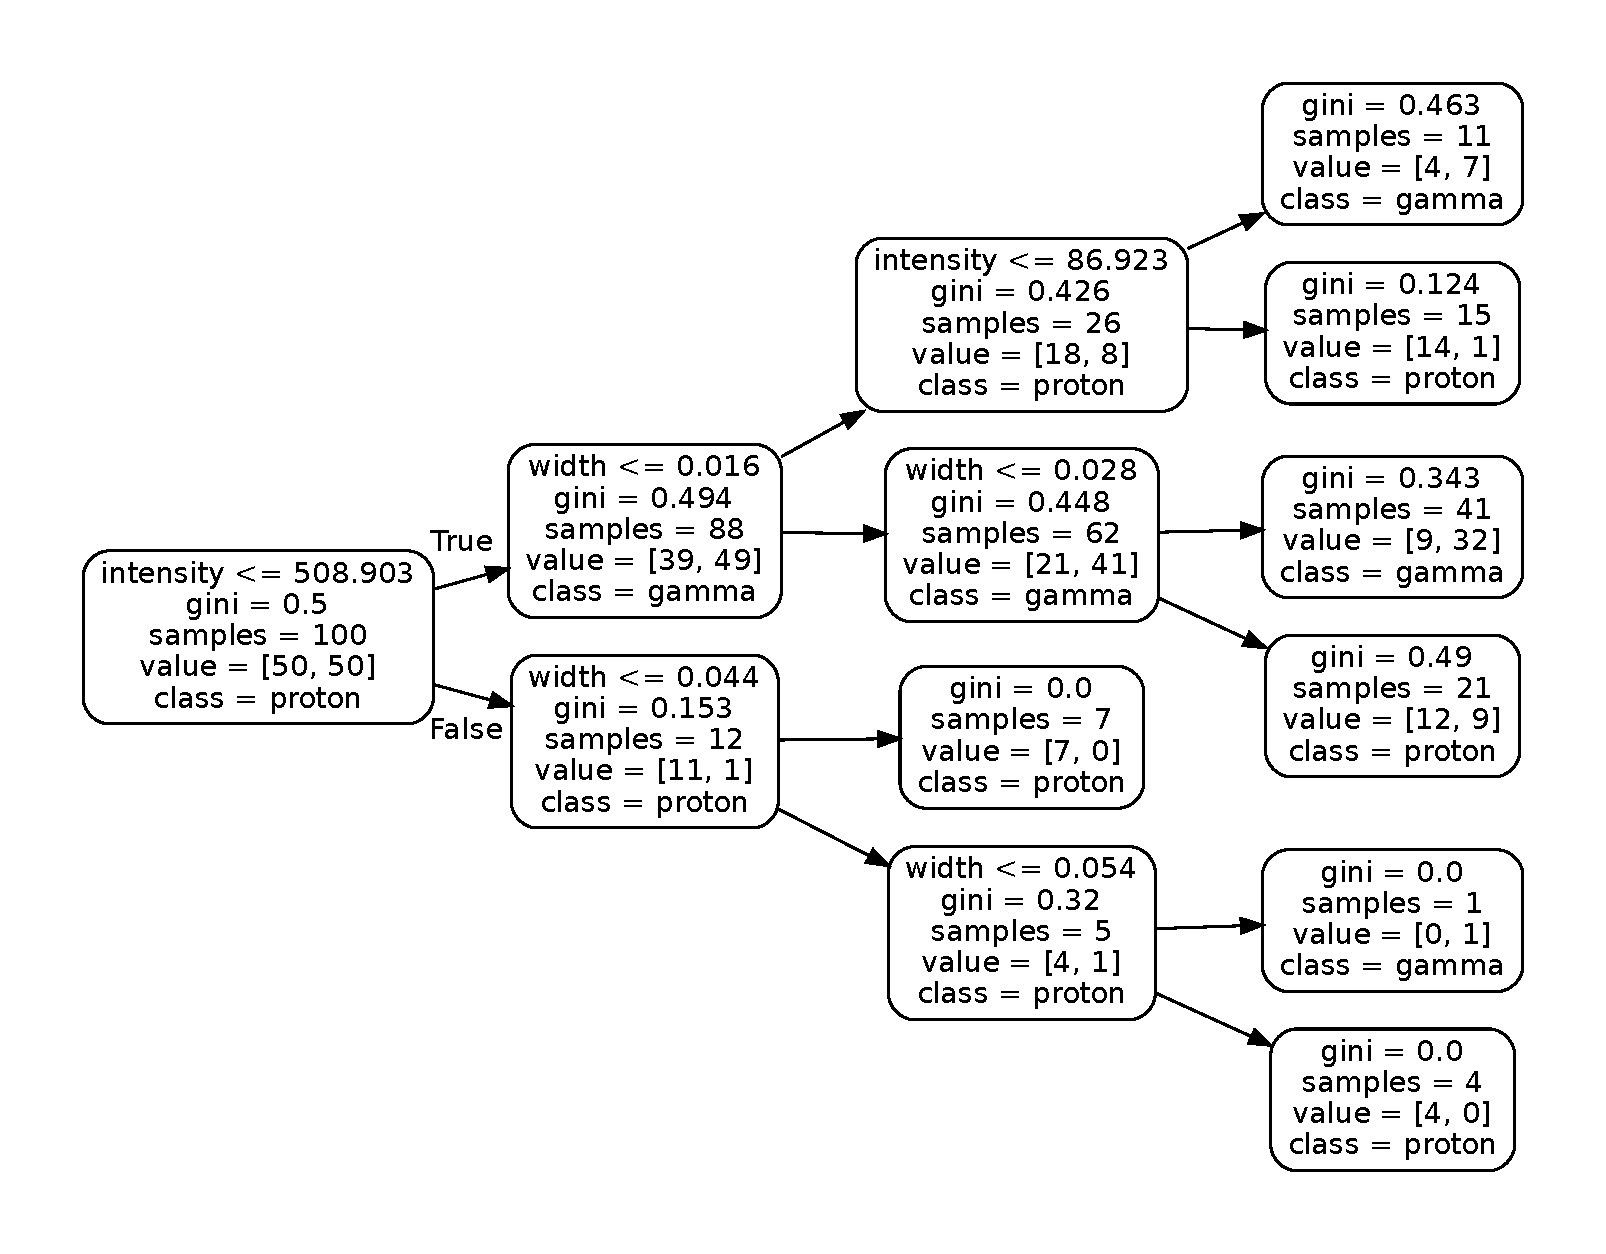
\includegraphics[width=0.8\textwidth]{Plots/decision_tree.pdf}
  \caption{A decision tree for a small sample dataset consisting of 50 proton and
  50 gamma events. The tree is capped at a depth of 4 and splits only on the 
  features width, length and intensity. On the training data, this tree reaches an
  accuracy of \num{0.81}.}
  \label{fig:03_tree}
\end{figure}


The implementation in sklearn is based on the one by
Leo Breiman et al \cite{breimanclassification}.
A single tree performs binary splits $\Theta = (j, t_m)$
at each node $m$ in order to split
the data at node $Q$ into two subsets
$Q_\text{left}$
and
$Q_\text{right}$.
The split consists of a feature $j$ and a threshold $t_m$ and is
chosen in a way to minimize a given measure.
Features, that are more important for the predictions, will
thus appear at the top nodes of the tree.
A stopping criterion can be defined as the measure not improving anymore or
alternatively the tree can stop at a predefined depth to
avoid overly complex models.

For classification tasks this means reducing the class impurity in the node.
Sklearn uses the gini impurity \eqref{eq:gini} or the
cross-entropy \eqref{eq:entropy} to quantify the class impurity.

\begin{equation}
	\text{Gini impurity: } = \sum_{k=1}^K \hat{p}_{mk}(1-\hat{p}_{mk})
    \label{eq:gini}
\end{equation}

\begin{equation}
    \text{Cross-entropy: } = -\sum_{k=1}^K \hat{p}_{mk}\log{\hat{p}_{mk}},
    \label{eq:entropy}
\end{equation}

with $p_{mk}$ denoting the proportion of class $k$ in node $m$.


For regression tasks, scikit-learn uses the mean squared error
or mean absolute error and the same principles apply.

While decision trees have the benefit of providing
easily interpretable, low bias models there are some drawbacks to this
approach, namely \cite{hastie2017springer}:
\begin{itemize}
  \item{Instability, high variance}
  \item{Lack of Smoothness}
  \item{Difficulty in Capturing Additive Structure}.
\end{itemize}

One approach to reduce these problems is the construction of
random forests \cite{Breiman2001}.

The main idea behind random forests is to use multiple
decision trees to suppress the problems single trees have, while
keeping their advantages.
For this to work, the individual trees should not be correlated.
Consequently the trees cannot all be constructed the same way.
To make sure the individual trees
are somewhat independent from each other,
randomness gets introduced to the construction of each tree.
In random forests this is on the one hand achieved by giving each tree a
random subsample from the training data, obtained with bootstrapping \cite{efron1992bootstrap}.
Another source of randomness is to perform splits on a node
based on only a random subsample of the available features.

The prediction of the random forest in scikit learn is then the average of
the single tree predictions.
In the case of a classification task, the probabilistic predictions for each class
get averaged, before deciding on a class.


\subsection{Background Separation and Energy Estimation}
One important task, that ctapipe does not handle yet, is the classification of
the primary particle. As the analysis focuses on the gamma rays as signal, 
this simplifies to binary classification with the two labels signal(gamma) and
background(proton).

A random forest is trained
on telescope level with the features from \ref{sec:measuring}, including
the array wide features obtained with the
HillasReconstructor.
The class impurity is measured with the cross-entropy.
In addition, new features are generated, namely:

\begin{enumerate}
    \item $\texttt{area} = \texttt{width} \cdot \texttt{length}$
    \item $\texttt{width\_length} = 1 - (\texttt{width}/\texttt{length})$
    \item $\texttt{log\_size} = \log{(\texttt{intensity})}$
    \item $\texttt{log\_size\_area} = \log{(\texttt{intensity})} / (\texttt{width} \cdot \texttt{length})$
\end{enumerate}

A 3-fold cross validation is used during training.
The single telescope predictions get combined by
taking the mean of the single
predictions to provide a prediction for the complete array-event.

%\subsection{Energy Estimation}
Estimation of the primary particles energy is another task, which 
is handled via a random forest model. This time a
regressor model is trained with the same
set of features and optimizing the mean squared error.
The target feature, the monte carlo energy, gets log-transformed,
because the energy spans multiple decades. This helps
predicting lower energies by reducing the target space \cite{ba-lars}.

For the training of the models, the available data gets split up into training
and test data. Of the diffuse gamma events and the proton events, 25\% get
used for training. The remaining events aswell as the pointlike simulated events
get used for the analysis.
The background separation model gets trained with both the gamma
and proton events, the energy regressor is trained on gamma events
exclusively.

\subsection{The DISP-Method}
For the reconstruction of the source position
one possible way involves using the DISP-method,
which -- at its core -- predicts a point in the coordinates
of the telescope's camera as the true source position.

To get from a point in the camera image to the origin of the shower,
one needs to transform between different coordinate frames,
which in this case is done via ctapipe.
In the monoscopic case this involves the horizon frame 
and the camera frame.
The horizon frame is a spherical coordinate system with the two angles azimuth and altitude.
It is used to describe the position of stars and shower origins.
In ctapipe, the azimuth is oriented east of north and altitude from the horizon 
to the zenith.
The camera frame on the other hand is a 
2D cartesian with an orientation defined by the telescopes pointing.
It is used to describe the shower in the focal plane.
The two coordinates $x$ and $y$ define a point in the focal plane,
with $x=0, y=0$ the camera center. 
% The telescope orientation is defined as 
% starting at the horizon, then pointed to the 
% magnetic north in azimuth and up to the zenith.
% The two coordinates are defined as they are in CORSIKA:
% $y$ points north and $y$ points west.

For stereoscopic reconstruction, a third coordinate frame has to be introduced.
The nominal frame describes a common, spherical frame for all telescopes.
It is necessary to use this frame, because the individual camera frames 
in general have different pointings.

The DISP-method assumes that the 
center of gravity of the shower image is displaced relative to the
real source position depending on the angle the shower was observed at.
If one assumes the true source position to be on the main shower axis of the ellipse,
finding this position simplifies to finding a single point on the main shower axis, that 
can then be transformed to the horizon frame.

Monoscopic experiments, that make use of the DISP method, need to resolve the head-tail-ambiguity:
The DISP calculation itself only grants the distance between
cog and source position, leaving two possible points.
One way to solve this problem is to treat it as classification task with two
classes $\pm1$, denoting the two directions to move from the cog.

Stereoscopic experiments can resolve this ambiguity by combining the images from 
multiple telescopes, as can be seen in figure \ref{fig:stereo_shower}.

\begin{figure}
	\centering
	\captionsetup{width=0.9\linewidth}
	\hspace*{0.1\textwidth}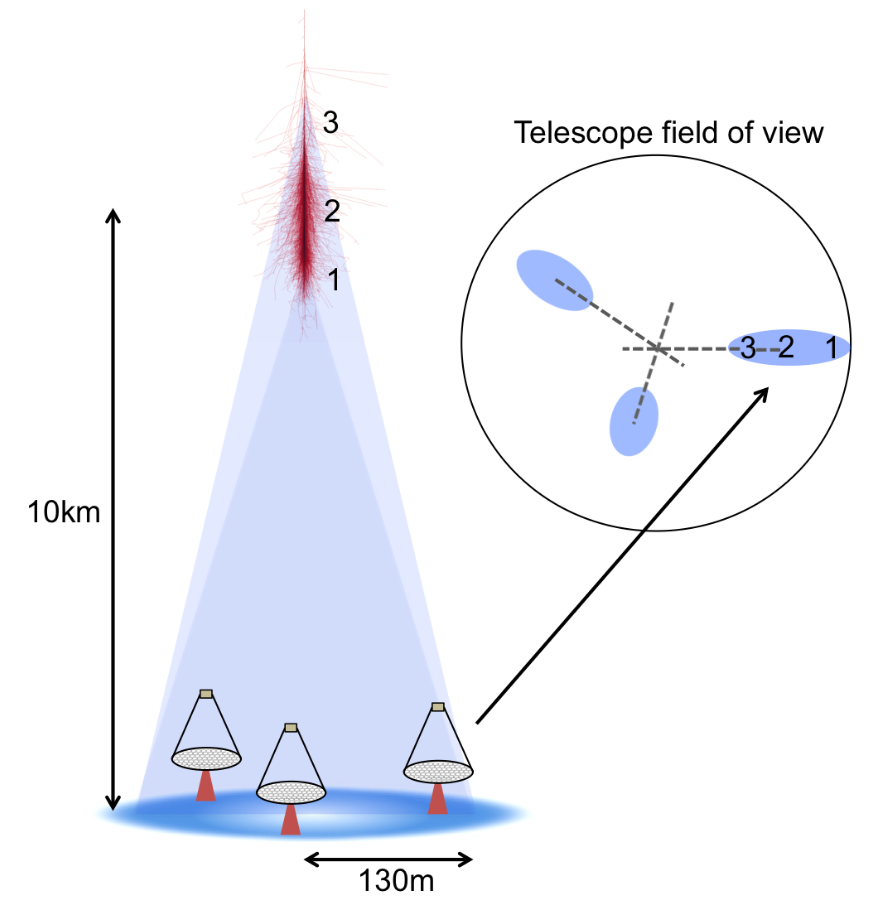
\includegraphics[width=0.7\textwidth]{images/stereo_shower.png}
	\caption{An illustration of an air shower captured with multiple telescopes.
		Each telescope captures an elliptic image.
		The image axes get intersected to reconstruct the arrival direction
		of the primary particle \cite{2015arXiv151005675H}.}
	\label{fig:stereo_shower}
\end{figure}


% The position on the shower axis can be estimated based on 
% the hillas parameters and other image features, as 
% explained in section \ref{sec:measuring}.

The calculation of the DISP is performed with a random
forest regressor model, based on the same features as before and
trained on the diffuse gamma training set.
To resolve the head/tail ambiguity in monoscopic mode,
a second random forest, a SIGN-model is trained.
In both cases a 5-fold cross validation is used.
The monoscopic prediction is then the chosen point in camera coordinates transformed
into the horizon frame.

Combining the individual results to an array wide predictions
involves a transformation of the telescope level predictions to
the nominal frame.
As a baseline estimation for the stereoscopic reconstruction,
the median of the single predictions in the nominal frame gets calculated
and transformed to the horizon frame afterwards.

Additionaly, an approach inspired by 
what the MAGIC collaboration does in some of their analyses,
is getting applied.
In the case of the MAGIC- xperiment the ambiguity does not
get resolved until the individual results are combined
at the stereo level. The choice of the correct
pair out of the four reconstructed positions can be done either
by calculating the crossing point of both main shower axes
or by calculating the pairwise distances between the positions.
At MAGIC, events where the minimum distance between the two points is larger than a set threshold
get discarded \cite{ALEKSIC201676}.

The method where all four distances are calculated is illustrated in figure \ref{fig:disp_magic}

\begin{figure}
    \centering
    \captionsetup{width=0.9\linewidth}
    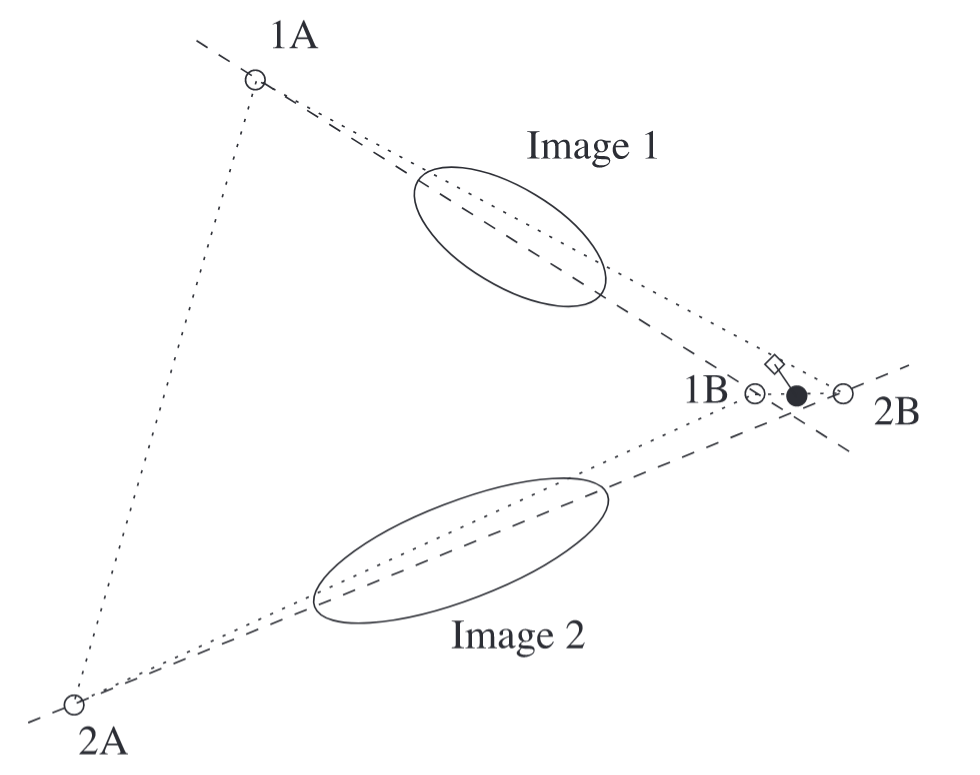
\includegraphics[width=0.7\textwidth]{images/magic_stereo_disp.png}
    \caption{Illustration of the stereoscopic DISP-reconstruction used in MAGIC.
        Two shower ellipses are drawn with the respective main shower axes as dashed lines
        and the two disp predictions each marked as 1A, 1B, 2A, 2B.
        The pairwise distances are displayed by the dotted lines.
        The closest pair is 1B-2B, the resulting prediction is calculated as 
        weighted average between the two points. The true source position is
        marked with a diamond \cite{ALEKSIC201676}.}
    \label{fig:disp_magic}
\end{figure}


Since CTA has more than two telescopes and each array event has a varying number
of associated telescope events, the method needs to be adapted in a scalable way.

The chosen approach is an iterative one:
For each pair of triggered telescopes, the results are combined
calculating the pairwise distances, as described in figure \ref{fig:disp_magic}. 

Distant events do not get discarded, because choosing an optimal threshold 
was found to be nontrivial and exceed the available time for the thesis.

From the research done, it seems to have little to no positive effect to weight
the average of the two points based on common image features such as 
the intensity or size, which is why an unweighted mean is used.

Figure \ref{fig:stereo_disp} illustrates this method for the case of 4 triggered telescopes.

\begin{figure}
    \centering
    \captionsetup{width=0.9\linewidth}
    \begin{subfigure}{0.45\textwidth}
        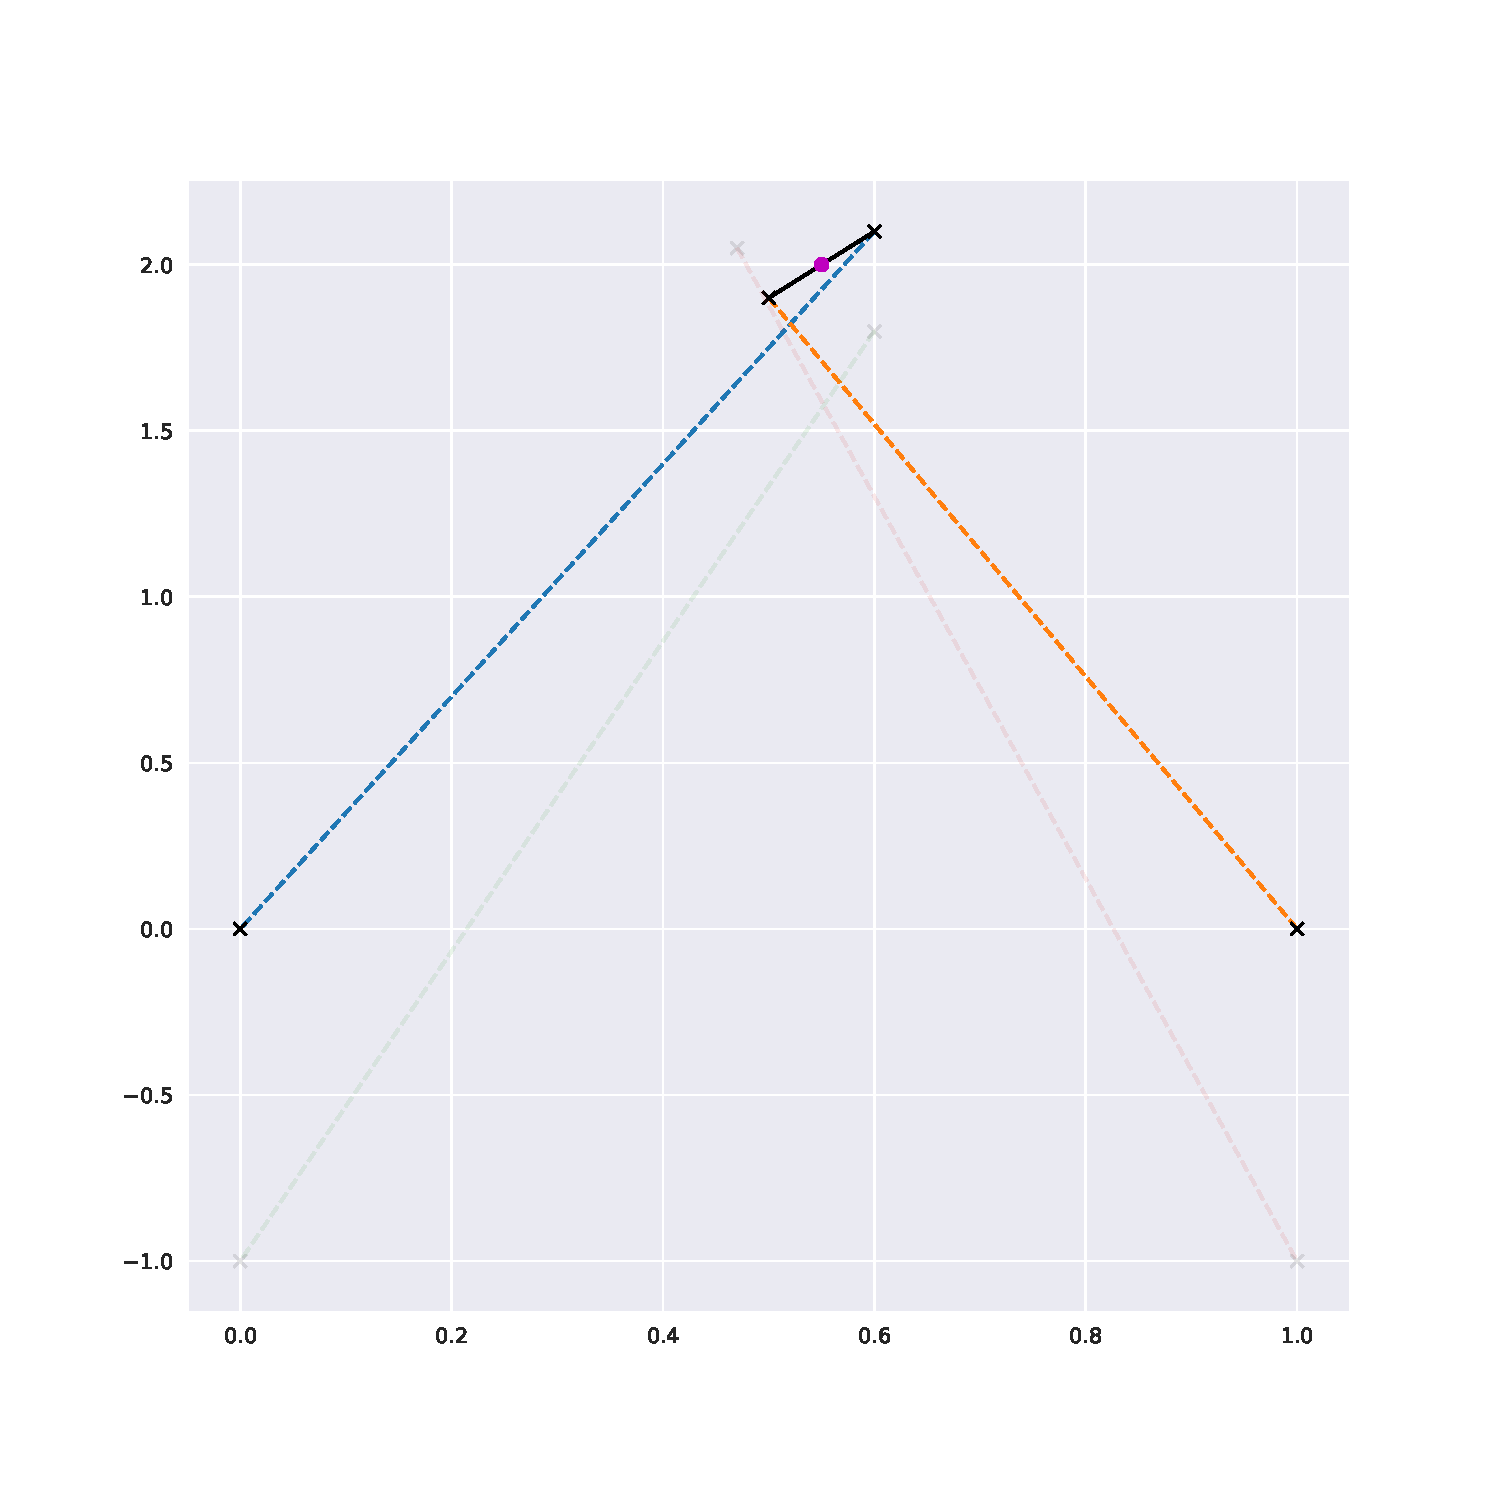
\includegraphics[width=\linewidth]{Plots/stereo_magic_1.pdf}
        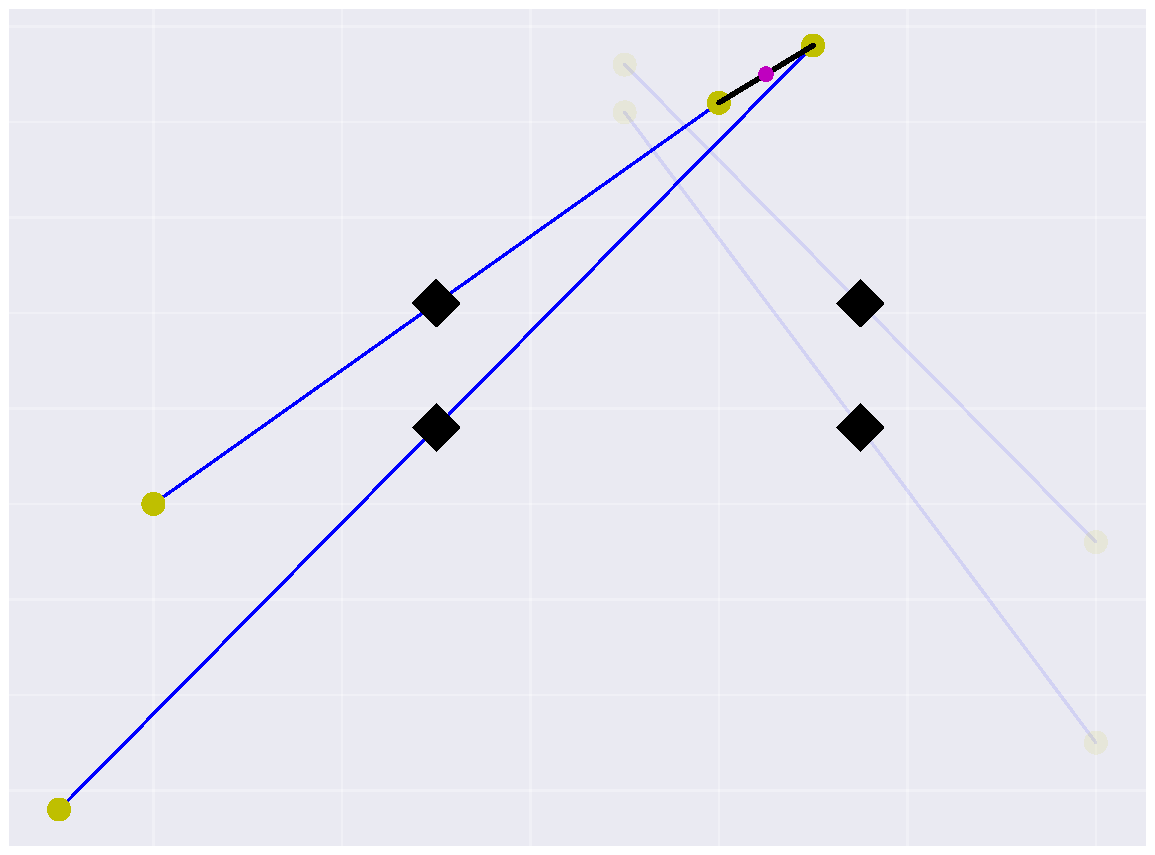
\includegraphics[width=\linewidth]{Plots/stereo_magic_2.pdf}
        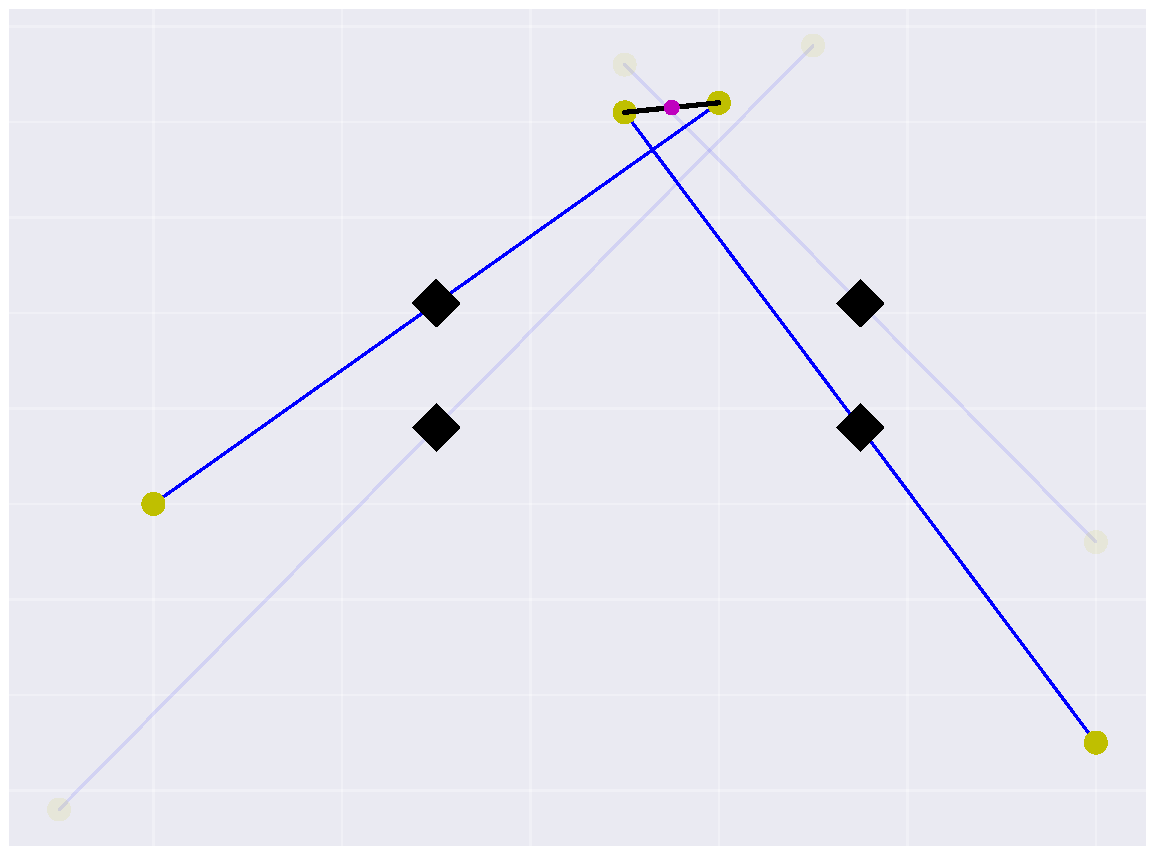
\includegraphics[width=\linewidth]{Plots/stereo_magic_3.pdf}
    \end{subfigure}
    \begin{subfigure}{0.45\textwidth}
        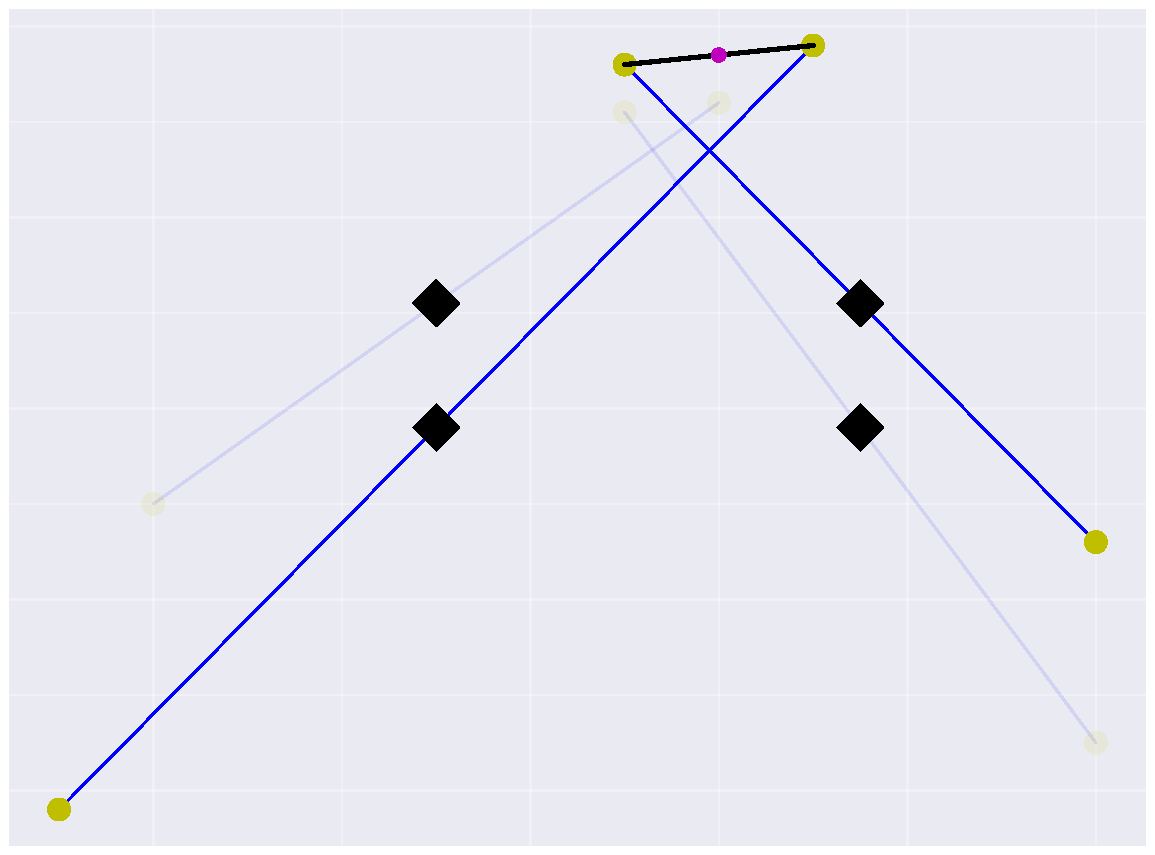
\includegraphics[width=\linewidth]{Plots/stereo_magic_4.pdf}
        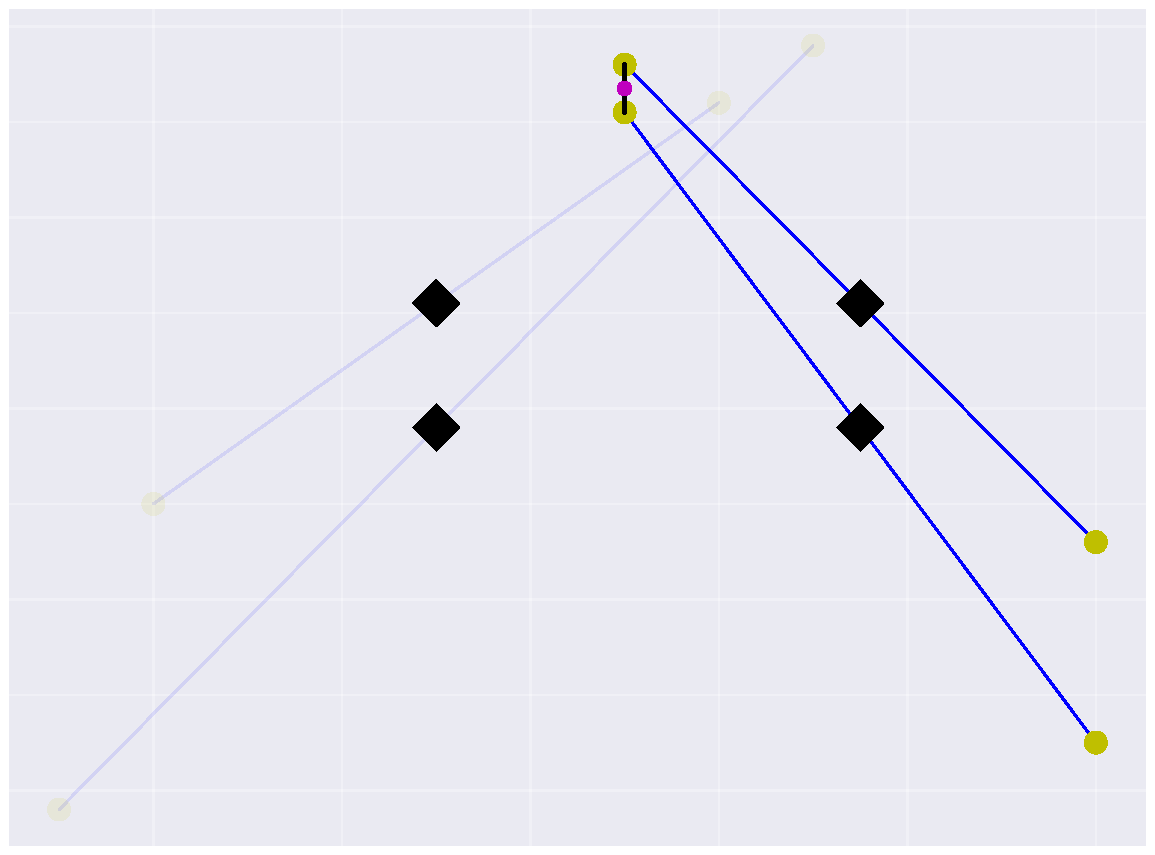
\includegraphics[width=\linewidth]{Plots/stereo_magic_5.pdf} 
        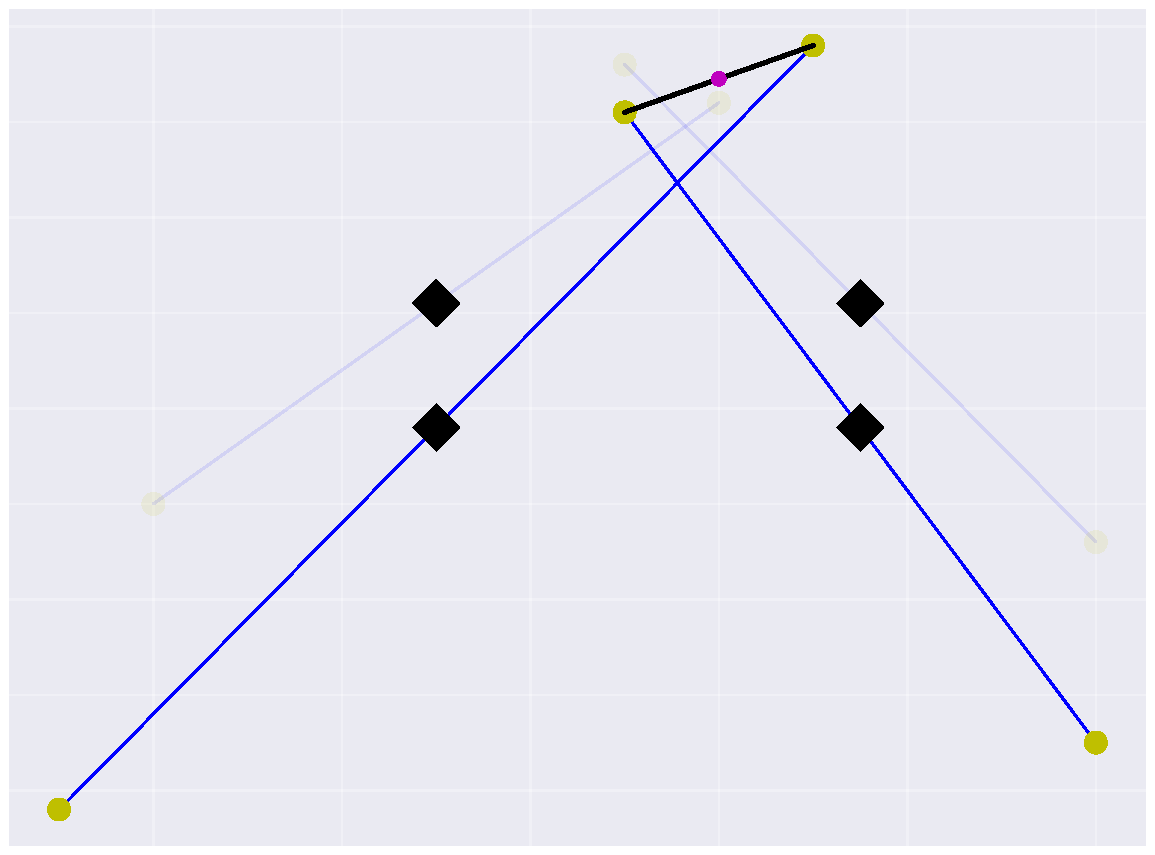
\includegraphics[width=\linewidth]{Plots/stereo_magic_6.pdf} 
    \end{subfigure}
    \caption{
    Illustration of the iterative extension to the stereoscopic magic approach
    with the DISP-predictions as unfilled dots, the intermediate resulting prediction
    as filled dot and the true source position as unfilled diamond.
    Four telescopes have triggered, leading to a total of eight individual DISP-predictions.
    For each pair of telescopes, the four predictions get evaluated according to \cite{ALEKSIC201676}
    without dismissing poor events based on the minimum distance, leading to one 
    intermediate prediction per unique pair.
    Taking the median of the six intermediate results leads to the final prediction.}
    \label{fig:stereo_disp}
\end{figure}

All intermediate results are saved and averaged to get the final prediction.
In this case taking the median of the pairwise predictions seemed to be more robust
than the mean, weighted or unweighted.


\section{Optimizing the Sensitivity}
To quantify the results of the analysis and compare the 
DISP and HillasReconstructor results, the point source sensitivity 
curve gets calculated for both aproaches.
It describes the minimum flux required by the analysis to detect a point
source with a set significance in a given amount of time.
This requires making predictions on both signal and background events
and optimizing event selection criteria in order to provide the best sensitivity.
CTA sets the required significance at $5\sigma$ in 50h observation time.

To get interpretable results, the simulated data has to be 
aranged in a way, that resembles the observation of a real point source.
The first task lies in weighting the events according to their energy,
because the simulated spectra do not match the observed spectra for cosmic
and gamma rays. They are instead chosen in a way to improve on the
computation time.
Reweighting can be done with the available data of the monte carlo production,
namely the spectral index, maximum and minimum energy.
For the signal events this means, that the events get weighted in order
to follow the energy spectrum of the CrabNebula.
For the spectrum of the Crab Nebula, the parametrisation obtained by the MAGIC
collaboration are used \cite{aleksic2015measurement}.

The background, which for this analysis consists only of protons, 
on the other hand has to be weighted to the cosmic ray spectrum.
For this, measurements of Sanuki et al are used \cite{Sanuki_2000}.

The mentioned significance is the
Li\&Ma significance \cite{li1983analysis}.
\begin{equation}
    S = \sqrt{
        2N_\text{on}\ln
        \left(
            \frac{1+t_\alpha}{t_\alpha}
            \frac{N_\text{on}}{N_\text{on}+N_\text{off}}
        \right)
        N_\text{off}\ln
        \left(
            (1+t_\alpha)
            \frac{N_\text{off}}{N_\text{on}+N_\text{off}}
        \right)    
        }
    \label{eq:li_ma}
\end{equation}
The formula is given in \eqref{eq:li_ma}, with $N_\text{on}$
the counts in the on region, $N_\text{off}$ the counts in the off region
and $T_\alpha$ the observation time in the off region divided by the
observation time in the on region. The on region contains events from the
source as well as background events, the off region is assumed to contain only
background events. 

With full information available on the monte carlo data,
the counts in the on and off regions are simply defined as:
\begin{align*}
    N_\text{on} &= N_s + t_\alpha N_b \\
    N_\text{off} &= N_b.
\end{align*}

The relative sensitivity then is defined as the factor, by
which the signal events count has to be scaled to reach a significance
of 5$\sigma$. Multiplying this factor with the source flux gives 
a measure of the required flux in astophysical units.

The size of the on region $\Theta$ is one of the parameters to optimize.
Due to the high amounts of data, that would need to be simulated 
in order to obtain enough background events for a sensitivity curve,
the region, from which the background events are taken, is defined
with a constant radius of \SI{1}{\degree}.
This means the background region is bigger
than the signal region, requiring a scaling of the background
event counts by a factor of
$\frac{\Theta_\text{on}^{2}}{t_{\alpha}}$.

The other parameters for the event selection are lower tresholds on
the classification score and the event multiplicity.
Optimisation happens independently in each bin of energy
with respect to maximizing the sensitivity.

In addition, some constraints on the number of remaining events exist.
Following CTA guidelines, the number of signal counts or excess counts
has to be $>10$. It also has to be larger than five times the assumed uncertainty
of the background counts, which is set to $1\%$.










% Sensitivity Computation????